%!TEX root = ../main.tex
\doublespacing
\chapter{The intrinsic sizes of type III radio bursts and comparison to recent simulations.}
\label{chap:observations_vs_theory}
Recent developments in the modelling of radio waves in a turbulent corona have made predictions about source sizes that have not yet been qualitatively compared to interferometric observations. Scattering of radio waves off of density inhomogeneities in the solar corona is considered to be the dominant cause of the size and shape of radio bursts. By understanding scattering, the turbulent nature of processes that generate density inhomogeneities can be studied. Turbulence in the corona can give insight into how energy is transferred from large scale phenomena down to the microscales, potentially resulting in the million degree Kelvin temperatures that have puzzled solar physicists for decades. New models of radio wave scattering, therefore, are the first step to solving fundamental physical problems in the solar corona. However, unless the models agree with observations, their use is limited and as such, comparisons between models and observations are crucial. In this chapter I utilise the direct visibility fitting method described in Chapter \ref{chap:measuring_source_sizes} and apply it to 29 type III radio bursts observed with LOFAR from 10-90~MHz. Using a Markov Chain Monte Carlo (MCMC) fitting method, it is determined that these bursts have a mean size along the major and minor axis of FWHM\textsubscript{x} = 16.27~arcmin and FWHM\textsubscript{y} = 11.96~arcmin respectively. No trend of source size with respect to helioprojective angle is found, which is in contrast to predictions from state-of-the-art radio wave scattering models. I discuss reasons for this discrepancy and how improved imaging and additions to scattering models can be used to resolve them.
%This study suggests that although many are in agreement, further exploration of the parameters of scattering simulations are necessary before they can be used to predict the nature of coronal density inhomogeneities.

\section{Introduction}
\label{sec:obsvtheory_intro}
The computational modelling of radio wave scattering has seen considerable development over the 50-odd years since some of the first simulations by e.g. \cite{Fokker1965} and \cite{Steinberg1971}. The theory for these early works followed from a generalisation of \cite{Chandrasekhar1952}, as was discussed in Chapter \ref{chap:theory}, and was developed to explain the observations of radio burst source size, position, directivity (power received from source in some solid angle compared to power from an isotropic source in the same solid angle) and time profile. These models considered scattering of radio photons off of density inhomogeneities in the solar corona. Notably, each of these scattering events occurred at a small angle. Simulations of this kind fell out of favour by the mid 1980s and remained mostly dormant until \cite{Thejappa2007} investigated the source directivity and time profiles of bursts using a different power spectrum of isotropic density inhomogeneities. In the studies by e.g. \cite{Fokker1965} and \cite{Steinberg1971}, the inhomogeneities were assumed to have a Gaussian power spectrum. However, in the intervening 30 years knowledge of turbulence in the solar corona proved this assumption to be incorrect. As mentioned in Chapter \ref{chap:measuring_source_sizes}, \cite{Coles1989} collated the results of numerous experiments to give the following description of the density inhomogeneity power spectrum, shown in Figure \ref{fig:CH_density_spectrum}. At large scales, greater than a few hundred kilometres, the spectrum is well described with a power law index of -5/3, which agrees with the Kolmogorov description of turbulence \citep{Kolmogorov1941}. For scales smaller than these but greater than a few kilometres, the spectrum becomes shallower and is better described with a power law index of $\sim -1$. Finally, on the smallest scales less than a few kilometres the spectrum steepens again. This steepening has been interpreted as the scale at which energy is dissipated by turbulence. \cite{Coles1989} also found that this inner scale increases with heliocentric distance. \cite{Bastian1994} expanded on this description of the density inhomogeneity power spectrum and investigated the angular broadening of radio waves sources at centimetre wavelengths.

Comparisons between the models mentioned above and observations of radio bursts have also developed over time. \cite{Stewart1972} compared the observed positions of fundamental and harmonic emission and related it to the then contemporary scattering models \citep[e.g.][]{Fokker1965,Steinberg1971}. As our knowledge of solar turbulence and the power spectrum of density inhomogeneities improved so too did the instrumentation, allowing for more accurate observations of radio bursts and thus more accurate comparisons. In particular, radio interferometers such as LOFAR and the MWA have the angular resolution to investigate radio emission from both bursts \citep[e.g.][]{Zhang2020} and the quiet sun \citep[e.g.][]{Sharma2020}. 
%Data from space-craft has also been used to directly compare with the model of \cite{Thejappa2007}. \cite{Krupar2018} use observations from STEREO A and B to study the time profiles of type III radio bursts and find that these can be explained from Monte Carlo scattering simulations with a value for the relative r.m.s density fluctuations of $\varepsilon \sim 0.06-0.07$. This was expanded on by \cite{Krupar2020} who used data from Parker Solar Probe and found that $\varepsilon$ decreased with height in the solar wind.

The latest development in the modelling of radio wave scattering is by \cite{Kontar2019}. Rather than using the small scattering angle approximation of previous work, \cite{Kontar2019} build on the work of \cite{Arzner1999} and \cite{Bian2019}. In this approach, the effect of anisotropic density inhomogeneities is treated as photon diffusion in momentum space and the Hamiltonian equations for photon position and momentum can be solved iteratively to trace a photon's path. This allows for a continuous transition from weak to strong scattering, whereas previous work is limited to regime of small angle scattering. \cite{Kontar2019} assume a spherically symmetric corona with an anisotropic distribution of electron density fluctuations, with wavenumber $\mathbf{q}$, such that $q_\parallel$ is parallel to the local radial direction. They perform Monte Carlo simulations of photons emitted from a point source at $\omega = 1.1 \omega_p(R_s)$ via fundamental plasma emission at a distance $R_s$ and an electron density from the \cite{Parker1960} density model of a spherically symmetric corona with constant temperature. In the \cite{Kontar2019} model, the kinematic properties and arrival time of each photon was recorded at a predetermined distance from the burst source where scattering is considered negligible. An image was then created by projecting photons directed towards the observer back to the plane of the source. For a radio burst that would be observed at $\sim 35$~MHz ($f_p = \omega_p/2 \pi \sim 32$~MHz), \cite{Kontar2019} find that value for the root mean square (r.m.s) of density fluctuations $\varepsilon = 0.8$ and an anisotropy factor of $\alpha = 0.3$ are necessary to explain previous observations \citep{Kontar2017}. The effect of source location on the modelled image are also investigated and it is found that sources appear more elongated in solar latitude close to the disk limb than they do at disk centre. \cite{Kontar2019} determine that this effect is less evident when an anisotropy factor of $\alpha = 0.5$ is used.

The conclusions of \cite{Kontar2019} have not yet been qualitatively compared to observations of radio bursts. In particular, whether a relationship between the source size and its location on the solar disk exists is an easy test of the validity of recent modelling efforts. In order to verify this relationship, one can measure the source eccentricity at various heliographic longitudes. However, due to the effects of imaging algorithms on observed source size, extreme care must be taken in this regard. The approach taken here directly fits a 2D elliptical Gaussian to the interferomteric visibilities, thereby eliminating the need to produce images. Here I improve upon \cite{Murphy2021} by implementing a Markov Chain Monte Carlo fitting method to get a robust description of fitting uncertainties. The position and size of the burst in the minor and major axes (FWHM\textsubscript{x} and FWHM\textsubscript{y} respectively) can be determined from this fitting and used to calculate the eccentricity or ``aspect ratio"  of the burst i.e. FWHM\textsubscript{x}/FWHM\textsubscript{y}.
%In the following sections I describe how the size of the burst in the major and minor axes (FWHM\textsubscript{x} and FWHM\textsubscript{y} respectively) are determined from LOFAR observations and how their ``aspect ratio" i.e FWHM\textsubscript{x}/FWHM\textsubscript{y}, can be used to compare the observations with recent modelling simulations.

Observations of radio bursts contain information on the scattering effects of radio waves as they travel through the corona to the observer. The process that determines this scattering needs to be fully understood before information about the solar corona can be determined from observations of radio bursts.
By measuring the aspect ratio of type III bursts as a function of heliographic longitude, a direct comparison can be made to the predictions of state-of-the-art scattering simulations. If they are in agreement, we may be able to use information about the scattering effects on a source to remotely determine the physics of coronal plasma.
%ground based observations of radio bursts can be used to accurately determine the properties of coronal plasma.	

\section{Observations}
\label{obsvtheory_observations}
During the period 04 April 2019 to 14 April 2019 a type III storm occurred on the Sun. This storm was observed in the frequency range of 20 - 80~MHz using LOFAR in both tied-array and interferometric mode. Interferometric visibilities at a frequency of 30.47~MHz from 12:00 UTC - 13:00 UTC on April 4-8 and 11-14 are used for this study. During this time a large active region (AR) rotated across the solar disk. Figure \ref{fig:ar_evolve} shows the active region with NOAA identification number 12738 revolves onto the disk. The active region is first classified on 08 April 2019 as a unipolar sunspot under the Hale classification and evolves to a bipolar structure by 14 April 2019. Assuming type III radio bursts occur above this active region, it offers a perfect opportunity to study the variation of source size and shape with respect to position. The heliographic longitude of AR 12738 changes by $\sim 80^\circ$ from close to the limb on 08 April 2019 to close to disk centre on 14 April 2019. This is an ideal range to measure variability of source size with respect to longitude.

\begin{figure}
\centering
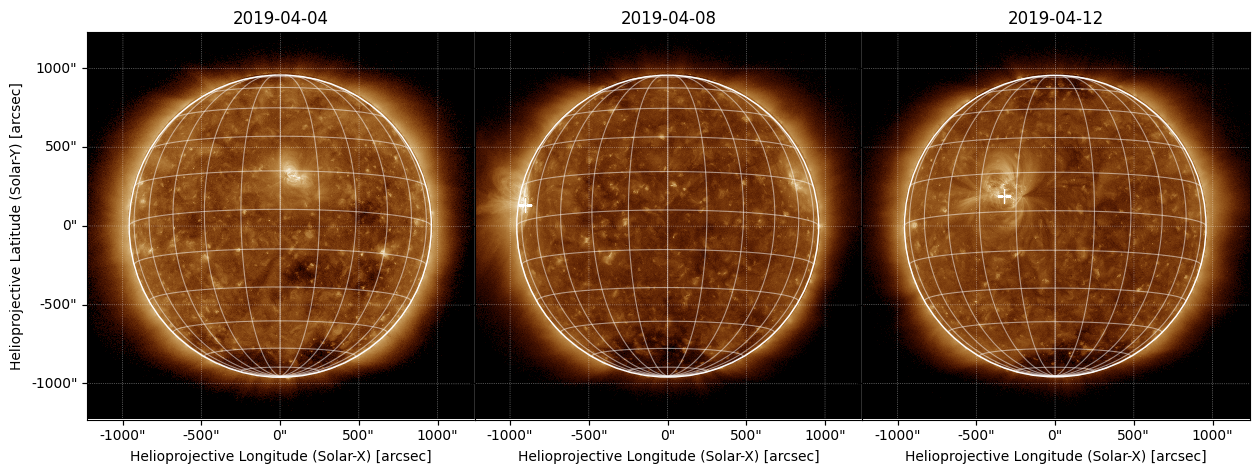
\includegraphics[width=\columnwidth]{aia193_ar_evolve.png}
\caption[Evolution of active region 12738 as it revolves around the disk.]{Evolution of active region 12738 as it revolves around the disk. Images are in the 193 \AA \ passband of AIA showing hot material in the solar corona. It is expected that type III bursts should be centred above the active region. The left panel shows the Sun on the first day of the observation where active region 12738 has not yet rotated onto disk. The middle panel shows the active region on the solar limb and is the first day where the active region is classified. The right panel shows the active region closer to the centre of the disk. In both the middle and right panel active region 12738 is marked with a white cross.}
\label{fig:ar_evolve}
\end{figure}

\section{Method}
\label{sec:obsvtheory_method}
The size and position of 29 type III radio bursts over the period of 04 April 2019 to 14 April 2019 were determined by directly fitting their interferometric visibilities. The bursts were identified in LOFAR beamformed observations and their peak time determined using an automatic peak finding algorithm. Peaks are found from the spectrum by first averaging over 16 subbands around 30~MHz, in order to match the spectral resolution of the interferometric observation, and smoothing the resulting time series. Then the \texttt{scipy} Python library \citep{Virtanen2020} is used to determine the peaks by comparing to neighbouring values. This list of peaks is filtered so that only peaks greater than the background plus five times the standard deviation are returned.
Figure \ref{fig:dynamic_spectrum_070419} shows the automatically identified bursts at 30~MHz. In total, 320 bursts were identified in this way. 

\begin{figure}
\centering
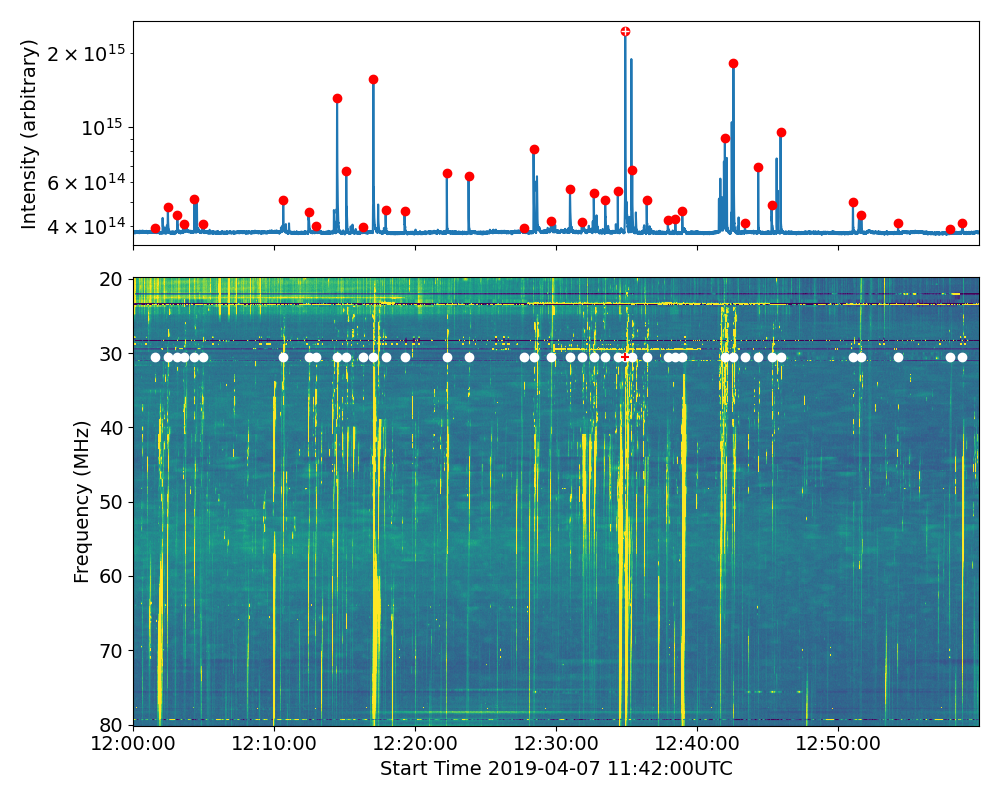
\includegraphics[width=\columnwidth]{peak_times_30MHz_wlightcurve_2019-04-07T120000_130000.png}
\caption[Type III storm observed on 07 April 2019.]{Type III storm observed on 07 April 2019. The top panel is the light curve at 30~MHz and the red dots indicate the detected peaks. The maximum peak is marked with a white cross. The bottom panel shows the dynamic spectrum of the storm. The white dots indicate the bursts identified by an automatic peak finding algorithm, the red cross indicates the brightest burst.}
\label{fig:dynamic_spectrum_070419}
\end{figure}

Unfortunately, due to the intensity of many radio bursts exceeding $\sim 500 kJy$, the calibration of interferometric data did not converge for $\sim 90 \%$ of them. This occurs when flux from the source is detected in the side lobes of the beam observing the calibrator. An example of burst visbilities with good and bad calibration solutions is shown in Figure \ref{fig:cal_comp}a and Figure \ref{fig:cal_comp}b respectively. 

\begin{figure}
\centering
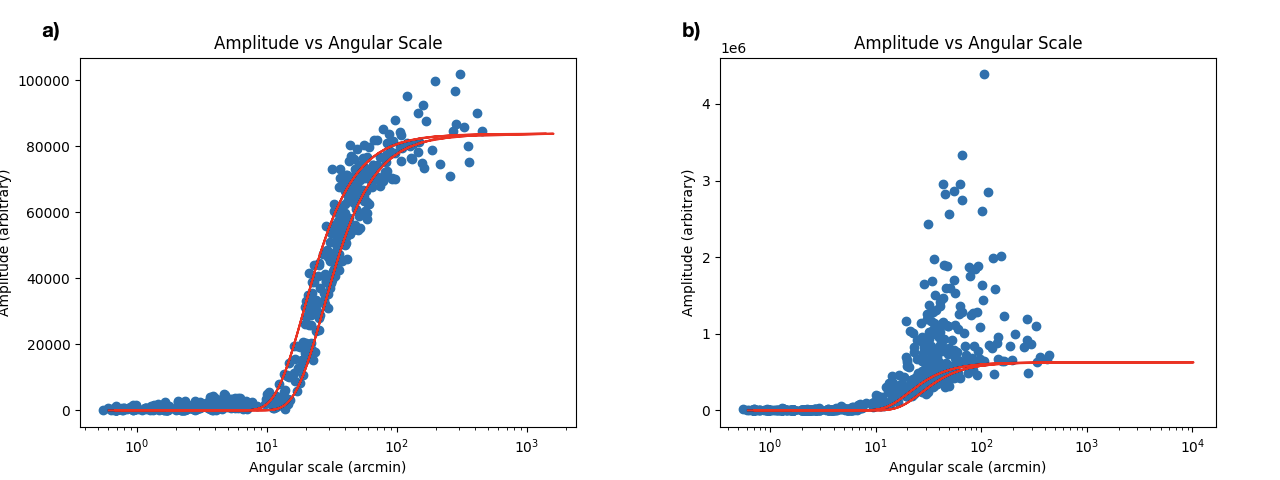
\includegraphics[width=\columnwidth]{cal_comp_vis.png}
\caption[Comparison of type III burst visibilities with good and bad calibration.]{Comparison of type III burst visibilities with good and bad calibration. Plotted are the amplitude of the burst visibilities with respect to angular scale in arcmin for a burst where calibtration did (a) and did not (b) converge. The red lines are the 2D Gaussian fitted to the visibilities.}
\label{fig:cal_comp}
\end{figure}

In order to determine the position and size of the identified bursts, their visibilities were fit with a 2D elliptical Gaussian at the time of the peak maximum. This makes the assumption that the burst is the only emitting source in the visibilities.
To estimate the error in each fit the probability distribution for the parameters determined. This can be done by employing a Markov Chain Monte Carlo (MCMC) technique. MCMC methods generate samples from a probability distribution, in this case the posterior probability density function of the fitting parameters, $x$, given the data, $D$,
\begin{equation}
\label{eq:pdf}
p(x \vert D) \propto p(x)p(D \vert x).
\end{equation}	
The most common form of MCMC algorithm is the Metropolis-Hastings (M-H) method which I will outline below. Starting at a particular state $x^{(t)}$ a proposed new state $x^\prime$ is drawn from some proposal density $Q(x^\prime;x^{(t)})$ which depends on the current state. $Q(x^\prime;x^{(t)})$ is a probability distribution from which it is easy to generate samples, such as a multivariate Gaussian. In order to determine whether or not to accept the new state the probability
\begin{equation}
\label{eq:MHnewstate}
a = \frac{p(x^\prime \vert D)}{p(x^{t} \vert D)} \frac{Q(x^\prime;x^{(t)})}{Q(x^{(t)};x^\prime)},
\end{equation}
is computed. If $a > 1$ the new state is accepted and the next iteration occurs. Otherwise the state is accepted with probability $a$. Note that if a state is not accepted, the position $x^{(t)}$ is repeated on the chain. Successive samples in a Markov chain are dependent meaning that it is only as $t \rightarrow \infty$, that the probability density function of $x^{(t)}$ tends towards $p(x \vert D)$. An improvement to the M-H algorithm which speeds up convergence is proposed by \cite{Goodman2010} and implemented in the \texttt{emcee} Python library \citep{Foreman-Mackey2012}. This method uses an ensemble of \textit{walkers} to determine the proposal distribution. For each walker $k$ in an ensemble of $K$ walkers, the proposed state is determined by the positions of the remaining $K-1$ walkers in the ensemble. To determine a move for the walker at $x_k^{(t)}$, a walker $x_j, j \neq k$ is chosen from the ensemble and the proposed move has the form
\begin{equation}
\label{eq:MCMC_walkers}
x_k^{(t)} \rightarrow x^\prime = x_j + Z(x_k^{(t)} - x_j).
\end{equation}
Here, $Z$ is a random variable drawn from the distribution
\begin{equation}
\label{eq:MCMC_g}
g(z) \propto 
\begin{cases}
\frac{1}{\sqrt{z}} & \mbox{if} z \in \left[\frac{1}{a}, a \right] \\
0 & \mbox{otherwise}
\end{cases}
\end{equation}
where $a$ is an adjustable parameter set to 2 by \cite{Goodman2010}. The probability of accepting a proposed step is given by
\begin{equation}
\label{eq:MCMC_stretch_newstate}
q = \min \left(1, Z^{N-1} \frac{p(x^\prime)}{p(x_k^{(t)})}\right),
\end{equation} 
where $N$ is the dimension of the parameter space. This process is then repeated in series for the remaining walkers in the ensemble.
The ensemble of walkers for each parameter in the 2D Gaussian which is being fit are show in Figure \ref{fig:MCMCchain}. Each black line represents a walker's individual Markov Chain and the cyan line is the mean of the ensemble. Here a ``burn-in" time of 500 steps was used to allow the walkers to explore the parameter space and ``forget" their initial position. This is a typical way to fine-tune an MCMC. 
\begin{figure}
\centering
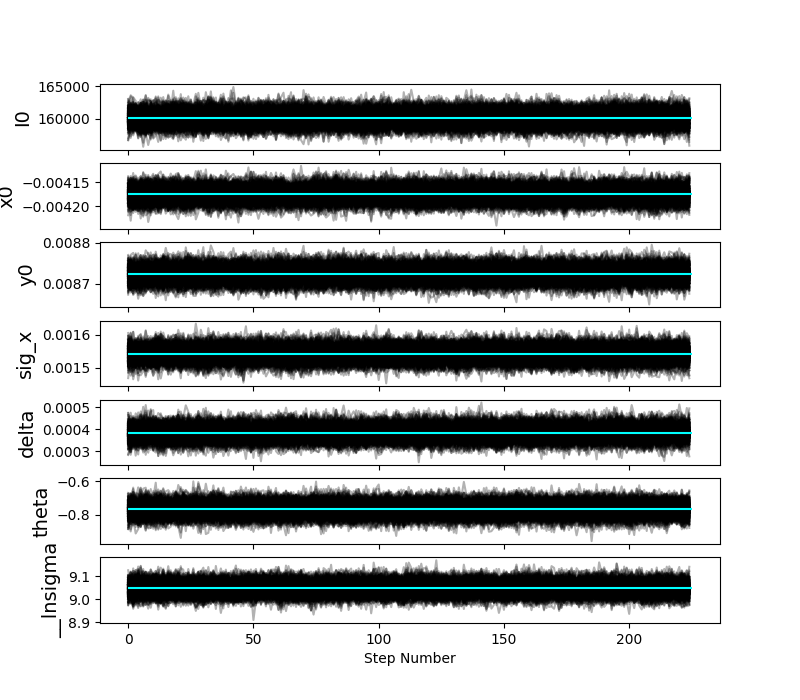
\includegraphics[width=\columnwidth]{chain2.png}
\caption[The Markov chain generated by 300 walkers for each parameter in visibility fitting.]{The Markov chain generated by 300 walkers for each parameter in visibility fitting. The parameters fit are as follows. \texttt{I0} is the amplitude of the Gaussian, \texttt{x0} and \texttt{y0} are the coordinates of its centre, \texttt{sig\_x} is the standard deviation of the Guassian in the x direction, \texttt{delta} is an additive factor to find the standard deviation of the Guassian in the y direction such that $\sigma_y = \sigma_x + \delta, \delta > 0$, \texttt{theta} is the position angle of the Gaussian and \texttt{\_\_lnsigma} is the log uncertainty of the visibilities. Horizontal cyan lines indicate the mean of the Markov Chain.}
\label{fig:MCMCchain}
\end{figure}

Once the MCMC has run for enough time to generate independent samples of the posterior probability density function, histograms of the samples can be projected into parameter space. The corner plot in Figure \ref{fig:MCMCcorner} shows the individual histograms as well as the 2D correlations between various parameters. This gives an excellent and robust measure of the error in each parameter.

\begin{figure}
\centering
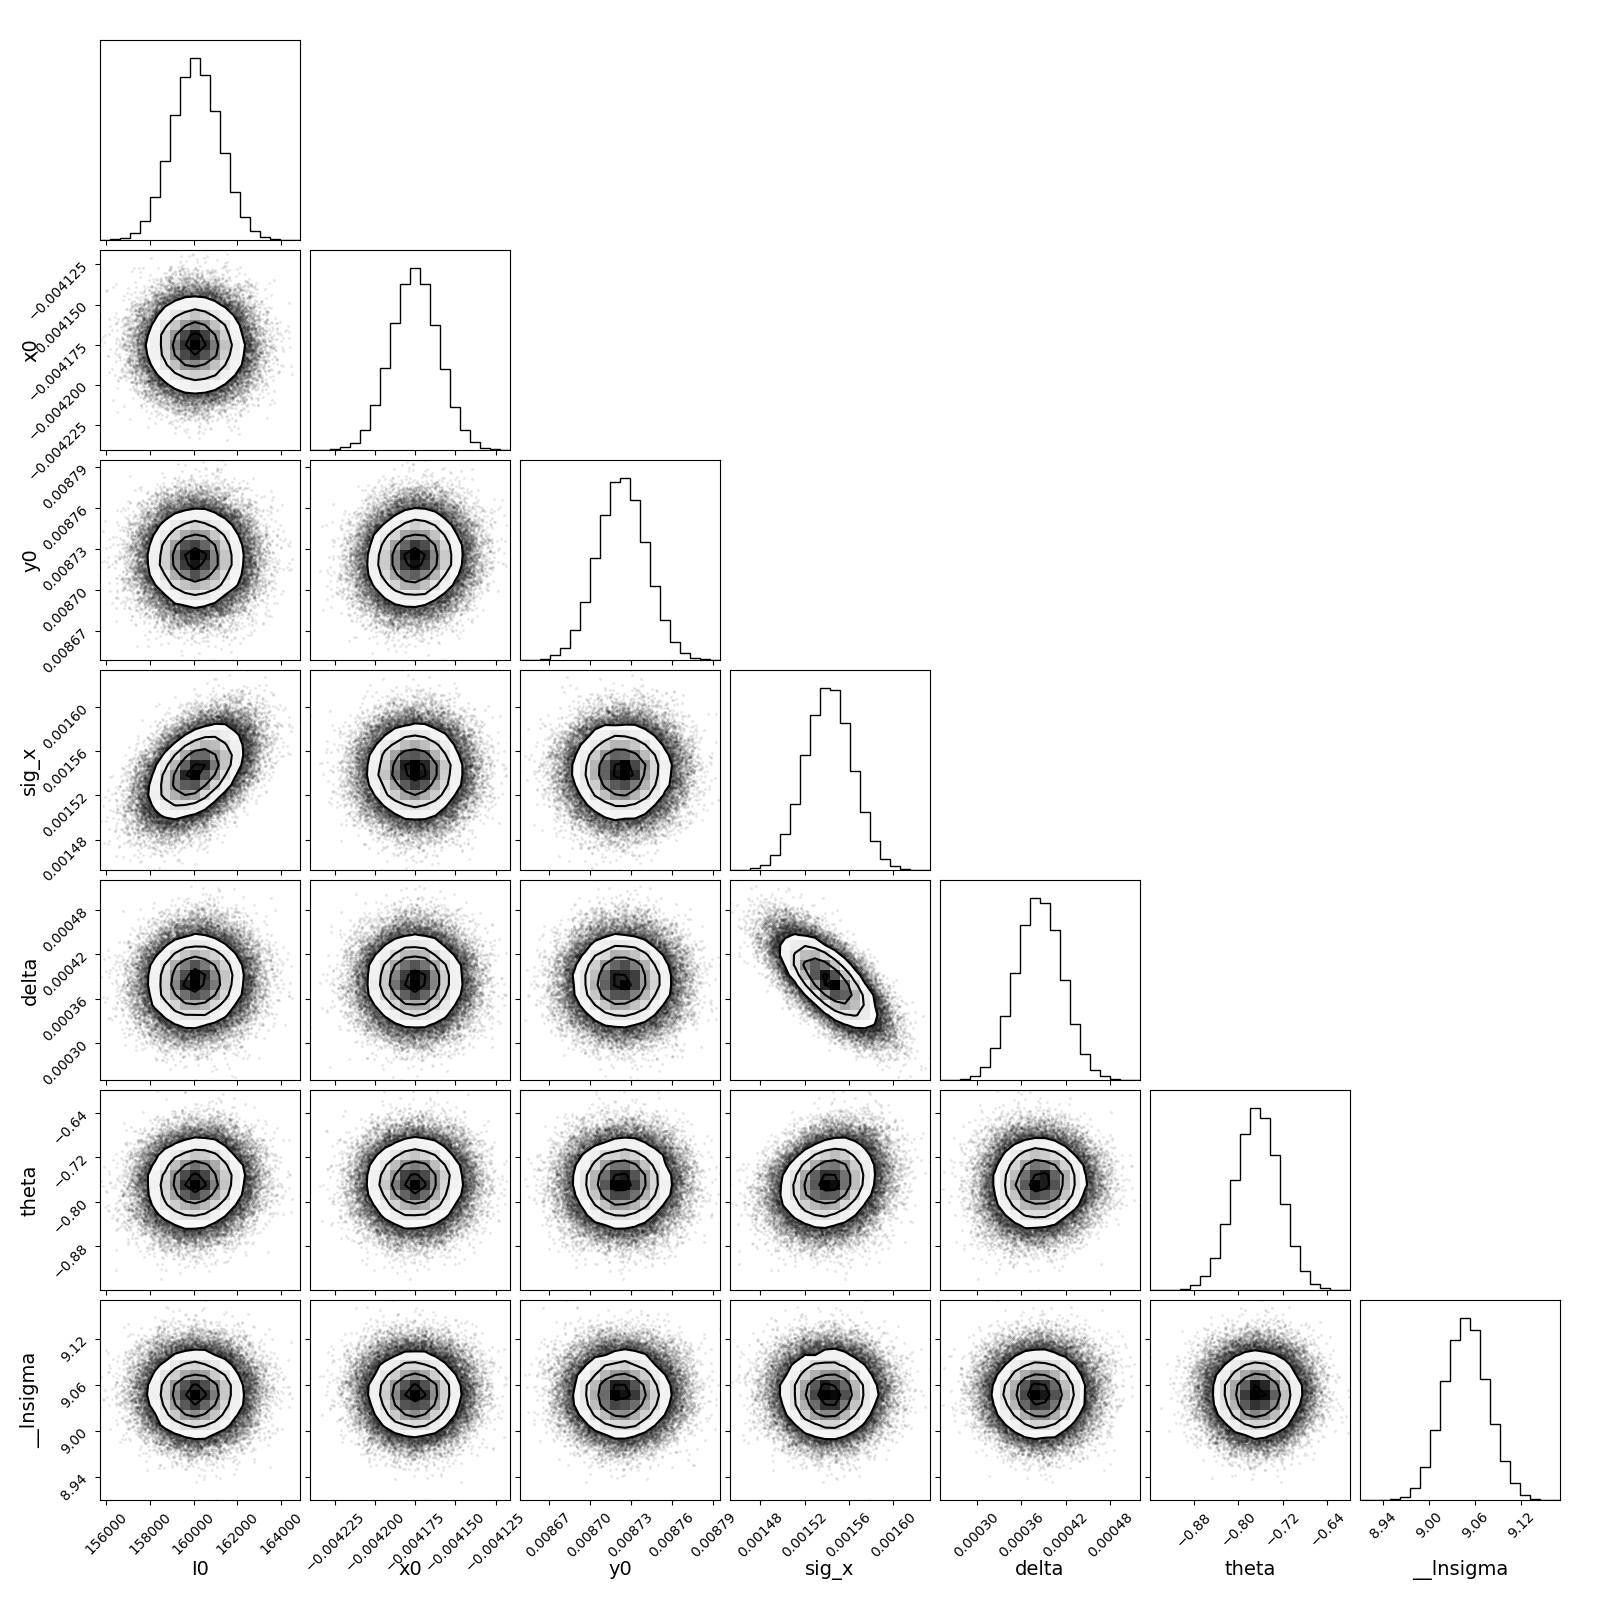
\includegraphics[width=\columnwidth]{corner2.png}
\caption[A corner plot of parameter histograms determined by MCMC algorithm.]{The corner plot of parameter histograms determined by MCMC algorithm. This shows the one (along the diagonal) and two dimensional projections of the sampled probability function. This can be used to determine the covariances between different parameters. The parameter labels are as described in the caption to Figure \ref{fig:MCMCchain}.}
\label{fig:MCMCcorner}
\end{figure}

The corner plots of all 320 identified bursts were manually inspected to identify cases where calibration succeeded. Any that did not show gaussian-like distributions such as in Figure \ref{fig:MCMCcorner} were deemed to have failed. Calibration was successful for 29 bursts.  

%As well as determining the source shape and position at its peak, the area of the source over its duration was also measured. This was done by fitting a straight line to the source area over the duration of the burst, which was estimated to be 1 second before its peak and 2 seconds afterwards.
The magnetic field structure around AR 12738 was determined by using a Potential Field Source Surface (PFSS) model using the Python library \texttt{pfsspy} \citep{Stansby2020}. This library solves the equations for magnetic field assuming there is no electrical field. Boundary conditions for the magnetic field are imposed from a spherical shell starting at the solar surface and ending at some configurable outer radius, 2.5 R$_\odot$ in this case.


\section{Results}
\label{sec:obsvtheory_results}
The parameters for all 29 fitted bursts are given in Table \ref{tab:dataset} where $I_0$ is the maximum intensity of the burst, $x_0$ and $y_0$ are the x and y  helioprojective-cartesian coordinates of the burst, FWHM\textsubscript{x} and FWHM\textsubscript{y} are the burst sizes along the minor and major axes of the Gaussian respectively and $\theta$ is the position angle of the fitted Gaussian. %Each fitted type III burst is plotted in helioprojective coordinates in Figure \ref{fig:burst_overlay}. It is clear from the figure that most bursts share a similar size and aspect ratio despite their relatively widespread origin in relation to the Sun's disk.

\begin{figure}
\centering
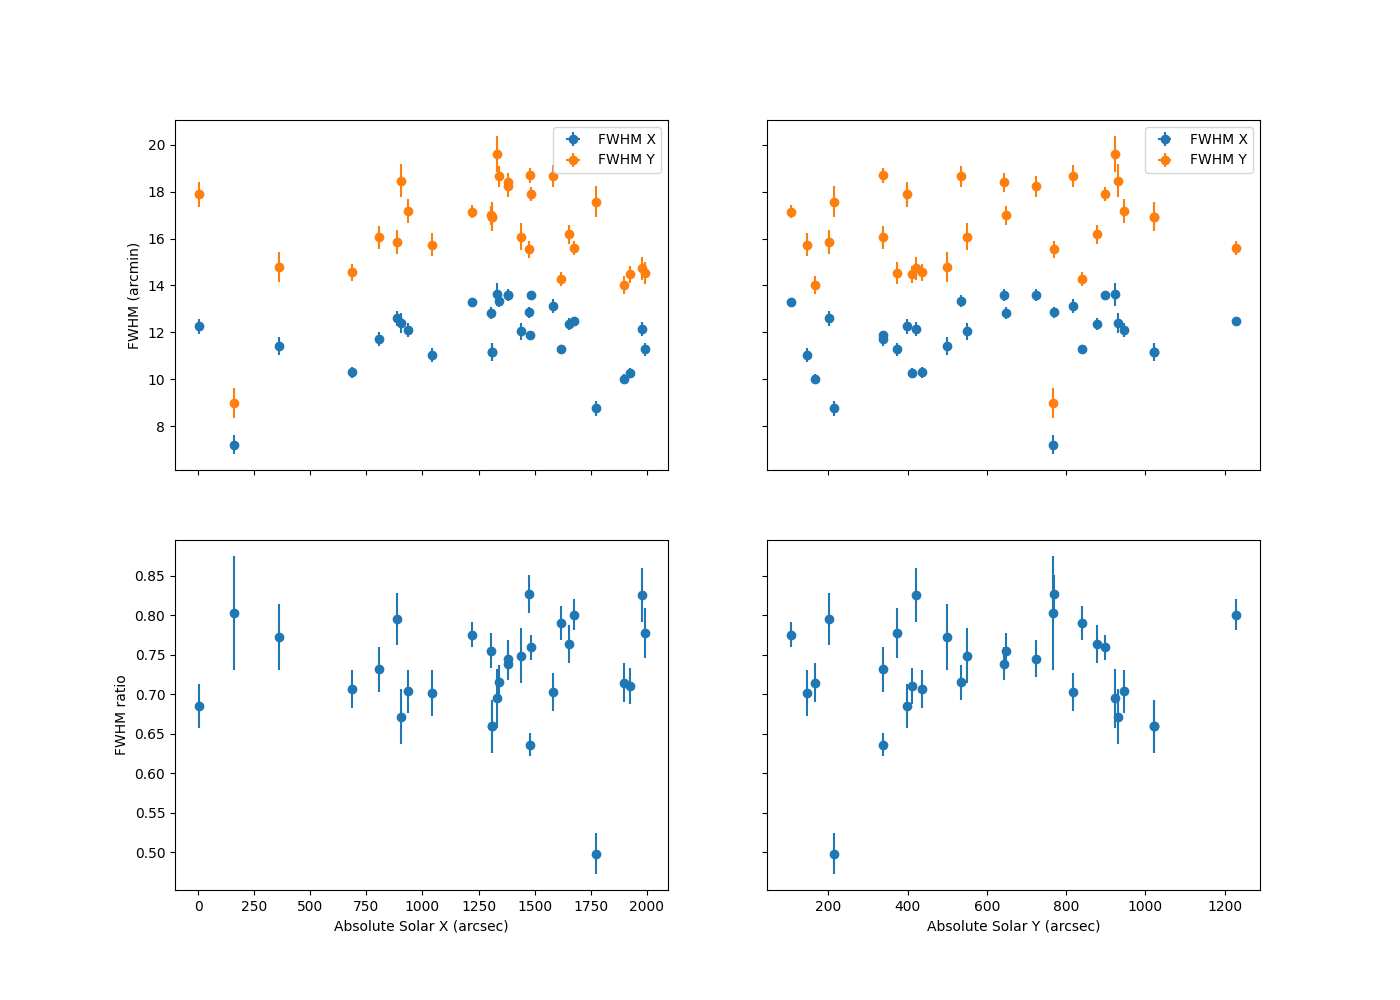
\includegraphics[width=\columnwidth]{fwhm_comparison.png}
\caption[Directly fitted type III burst sizes as a function of position relative to disk centre.]{A comparison of the directly fitted type III burst sizes and their distance from the disk centre in the helioprojective-cartesian x and y direction. Top row, FWHM\textsubscript{x} (blue) and FWHM\textsubscript{y} (orange) as a function of their absolute distance from the disk centre in the x (left) and y (right) direction. Bottom row, same as above except showing the ``aspect ratio" of each burst. There is no correlation with burst size or aspect ratio with respect to distance from disk centre either longitudinally (Absolute solar x) or latitudinally (Absolute Solar Y).}
\label{fig:fwhm_comp}
\end{figure}

\begin{figure}
\centering
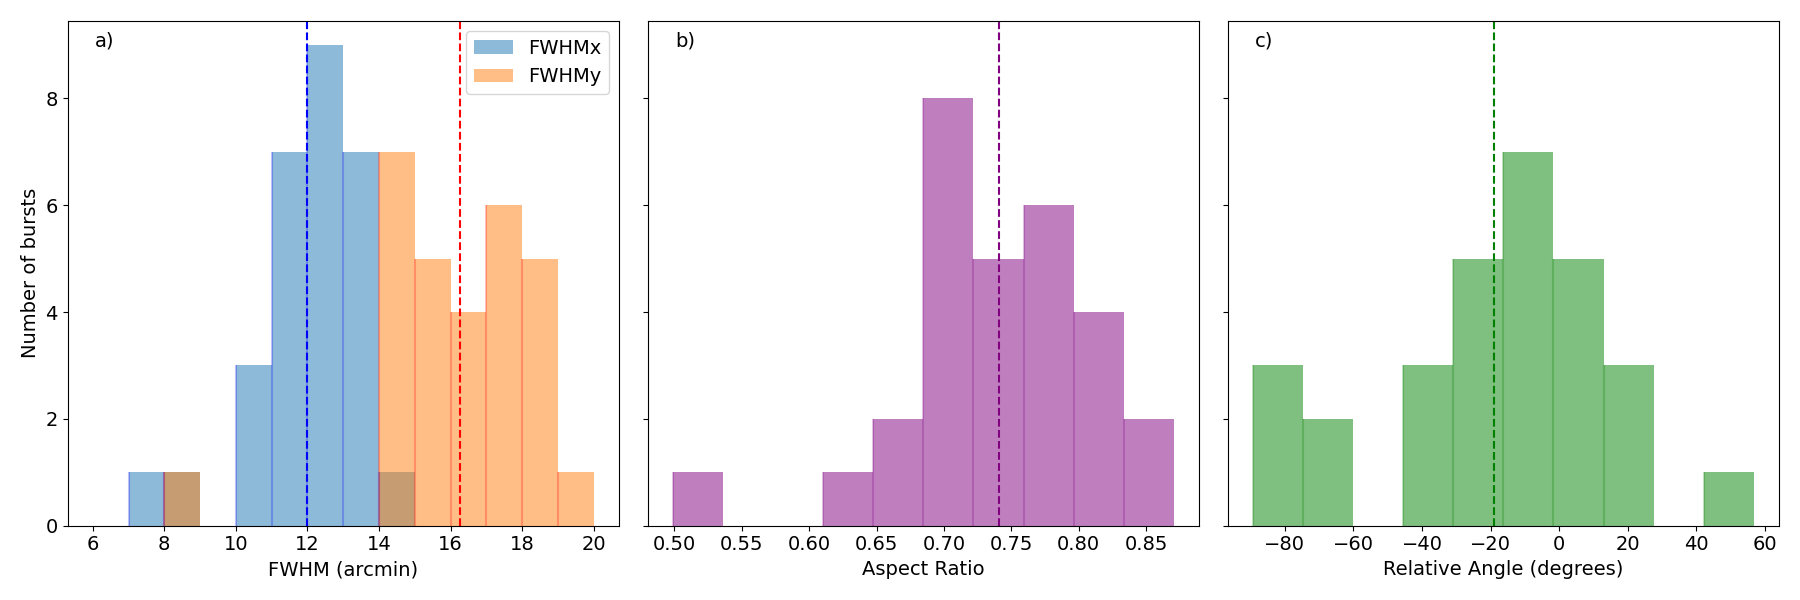
\includegraphics[width=\columnwidth]{burst_3histogram.png}
\caption[Histograms of type III burst sizes, aspect ratios and relative angles.]{a) Histogram of type III burst sizes. Bins are 1~arcmin wide and the vertical dashed lines indicate the mean value for FWHM\textsubscript{x} (blue) and FWHM\textsubscript{y} (orange). A peak in the FWHM\textsubscript{x} of the bursts could suggest an intrinsic size while the possible double peak in FWHM\textsubscript{y} shows that scattering effects cannot simply be determined from burst size alone. b) Histogram of type III burst aspect ratios. The vertical purple dashed line indicates the mean value for the aspect ratio FWHM\textsubscript{x}/FWHM\textsubscript{y}. A peak here possibly indicates that the observed aspect ratio depends more on the intrinsic size of a burst than the scattering effects. c) Histogram of type III burst relative angles. The vertical green dashed line indicates the mean value for the angle between the minor axis of the burst and a line joining its centre to (0,0). A peak near $0^\circ$ indicates a preference for bursts to be oriented perpendicular to the radial direction from disk centre. Observations of bursts in the solar winde support this suggestion \citep{Anantharamaiah1994,SasikumarRaja2016}. Large errors in the burst position angle for three bursts (Table \ref{tab:dataset}) can account for the outliers $< -80^\circ$.}
\label{fig:burst_hist}
\end{figure}
The size of each burst, is plotted against the distance from the disk centre in the helioprojective-cartesian x and y direction in Figure \ref{fig:fwhm_comp}. 
%There is no obvious trend towards bigger/smaller bursts with increasing distance from disk centre
% and, most strikingly, in direct contrast to the prediction by \cite{Kontar2019} 
There is no trend in the aspect ratio of the bursts, which is expected to be a linear decrease from 1 near disk centre to $< 1$ near the limb. 
%\begin{figure}[ht]
%\centering
%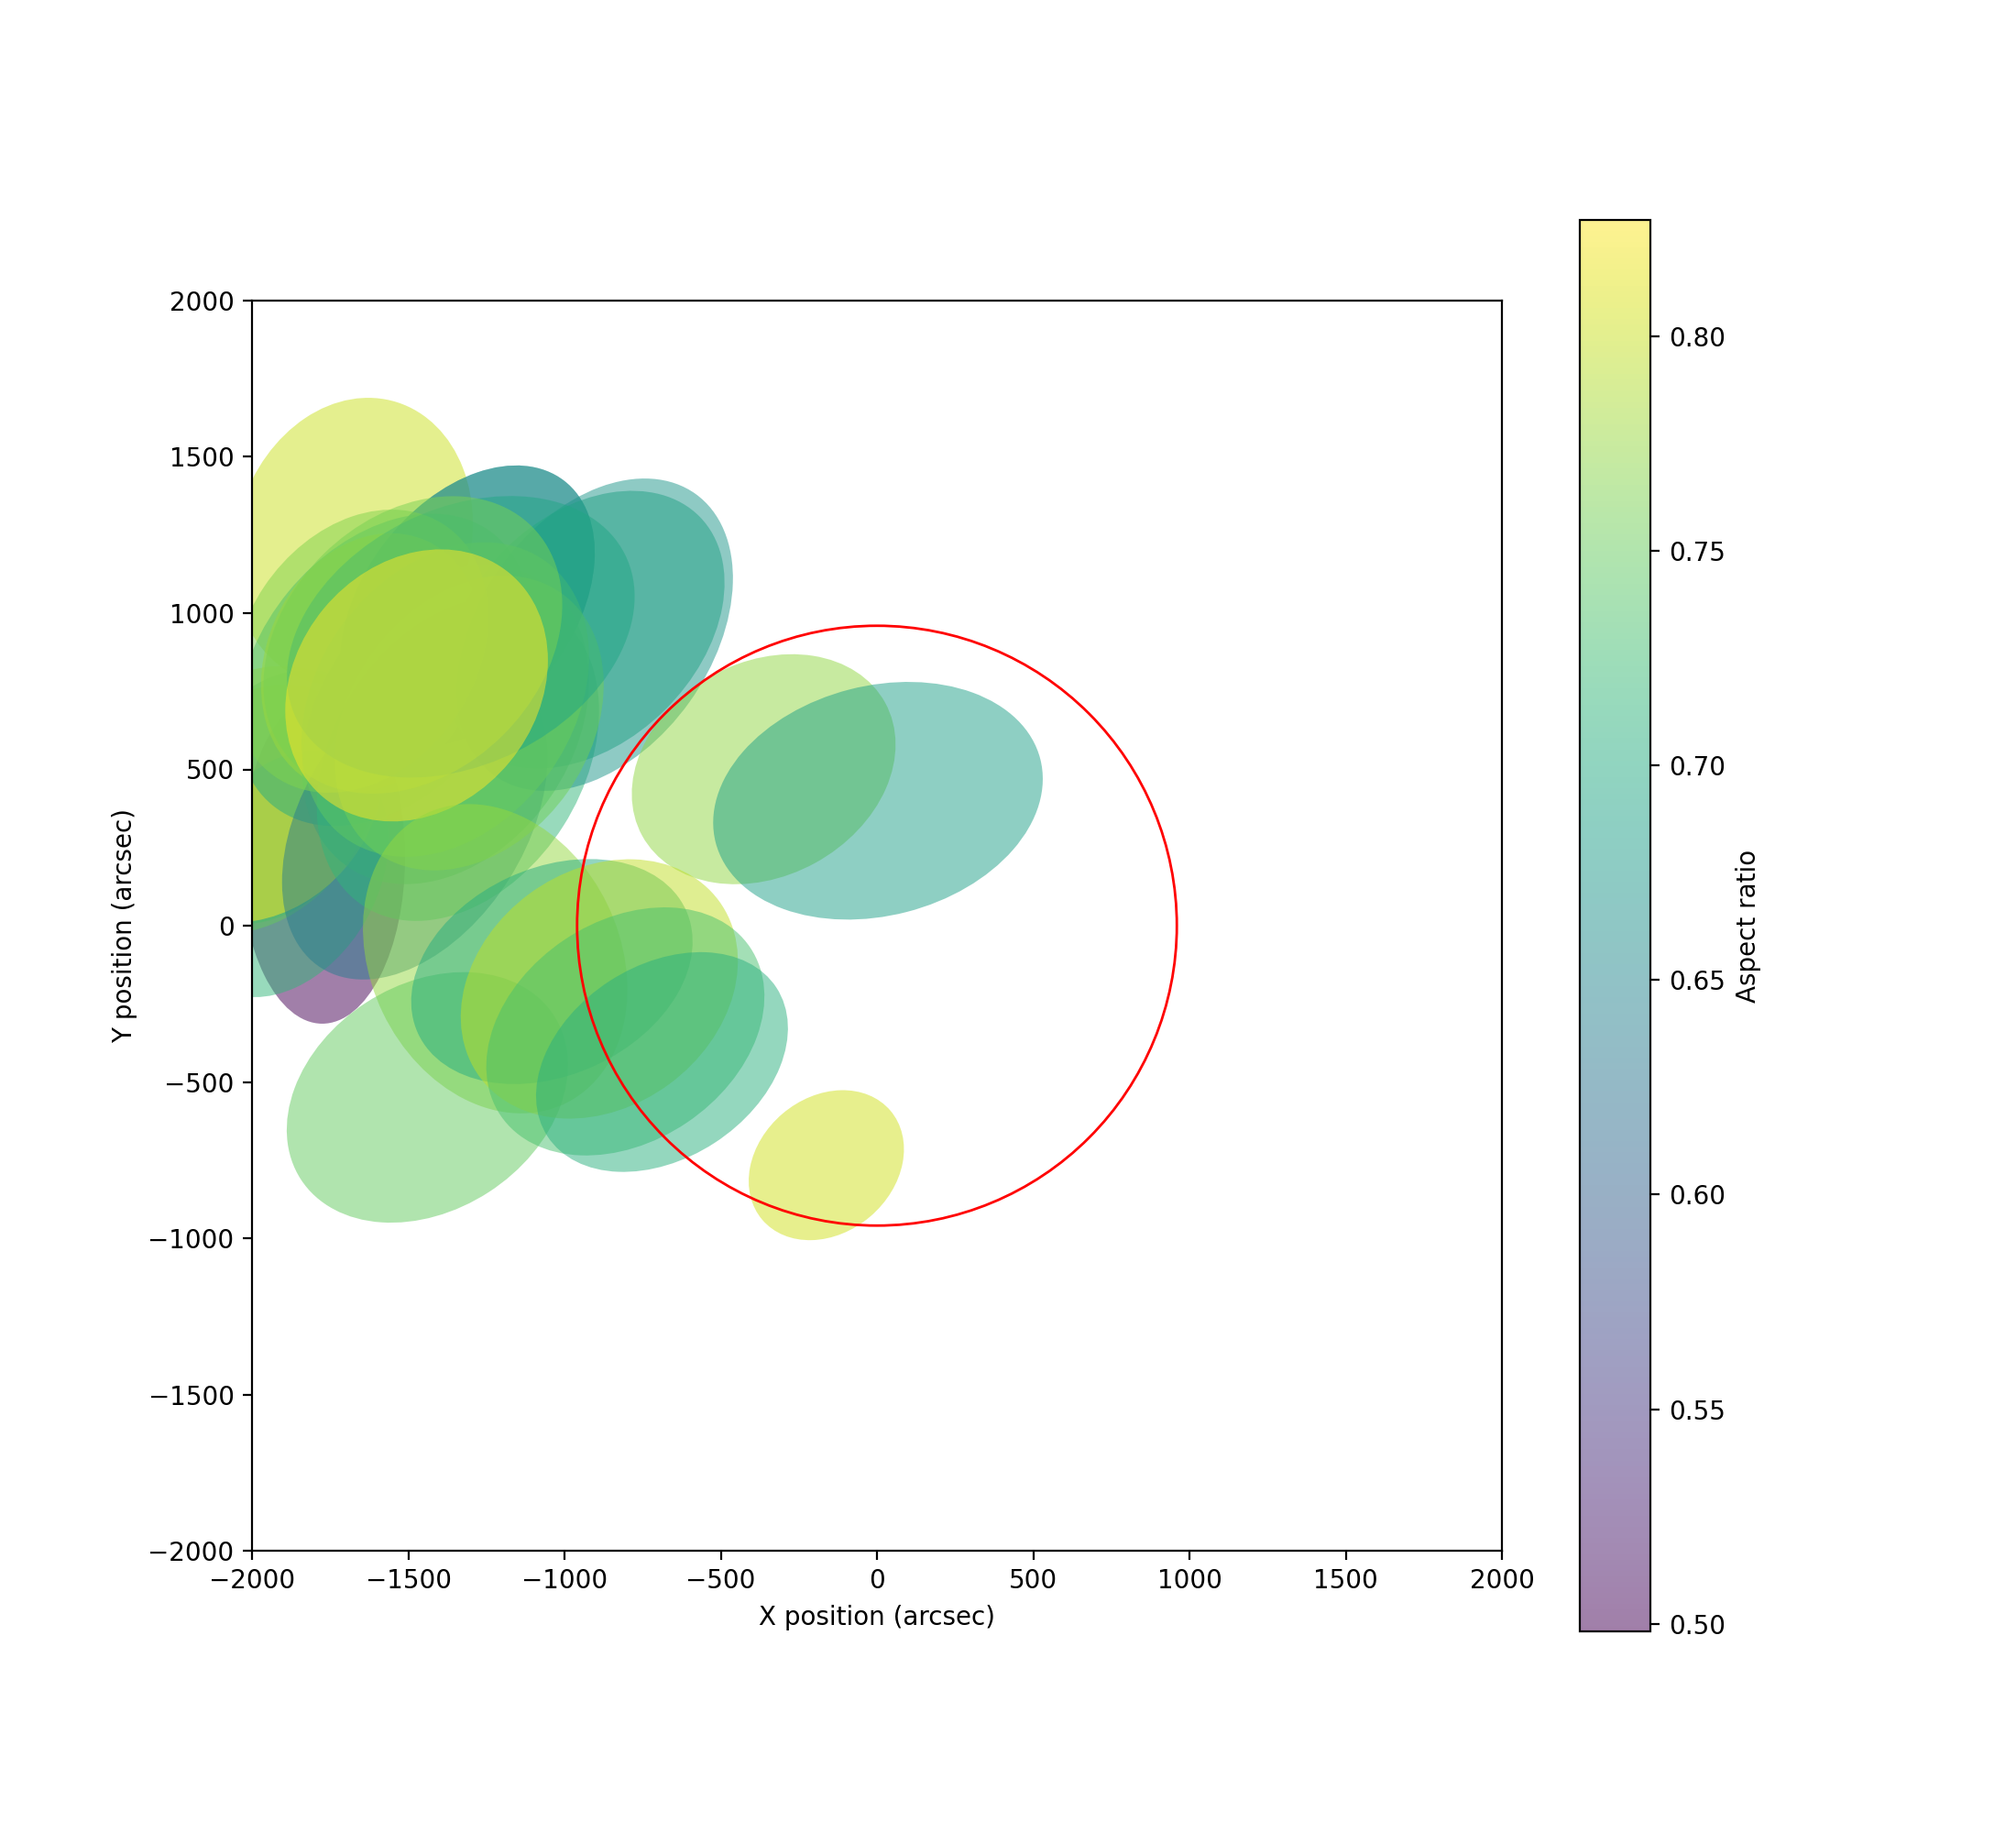
\includegraphics[width=\columnwidth]{burst_ellipses_best.png}
%\caption[Plot of type III radio bursts in helioprojecive coordinates.]{Plot of type III radio bursts in helioprojecive coordinates. Each ellipse has the size and location determined from direct visibility fitting. The colour of each ellipse is the aspect ratio. The red circle indicates the visible solar limb. }
%\label{fig:burst_overlay}
%\end{figure}

%\begin{landscape}
\begin{table}

\centering
\caption[Table of burst parameters from direct fitting to interferometric visibilities.]{Table of fitted burst parameters for each of the 29 bursts described in Section \ref{sec:obsvtheory_method} fitted with a 2D Gaussian in visibility space. The units in each column are given in brackets. Here $I_0$ is the maximum intensity of the burst, $x_0$ and $y_0$ are the x and y helioprojective coordinates of the burst, FWHM\textsubscript{x} and FWHM\textsubscript{y} are the burst sizes along the minor and major axes and $\theta$ is the position angle of the fitted Gaussian.}
\label{tab:dataset}
\sisetup{separate-uncertainty}
\begin{tabular}{lS[table-format=6.0(4)]S[table-format=+4.0(1)]S[table-format=+3.0(1)]S[table-format=2.1(1)]S[table-format=2.1(1)]S[table-format=+3.0(2)]}%p{\columnwidth}}
\toprule
Burst Time & {$I_0$}  & {$x_0$} & {$y_0$}  & {FWHM\textsubscript{x}} & {FWHM\textsubscript{y}} & {$\theta$} \\
 2019-04 & {(Jy)} & {(arcsec)} & {(arcsec)} & {(arcmin)} & {(arcmin)} &  {(deg)} \\
\midrule
05T12:08:08 &   90300 \pm 1310 & -1773 \pm 6  &   214 \pm 8  &    8.8 \pm 0.3 &   17.6 \pm 0.6 &  -27 \pm 2 \\
07T12:02:29 &   83800 \pm  678 & -1924 \pm 3  &   412 \pm 4  &   10.3 \pm 0.2 &   14.5 \pm 0.4 &  -55 \pm 2 \\
07T12:04:22 &  108000 \pm 1110 & -1990 \pm 5  &   372 \pm 5  &   11.3 \pm 0.3 &   14.5 \pm 0.5 &  -67 \pm 3 \\
07T12:15:08 &  160000 \pm 1100 & -1677 \pm 3  &  1229 \pm 4  &   12.5 \pm 0.2 &   15.6 \pm 0.3 &  -44 \pm 2 \\
07T12:31:00 &  120000 \pm 1010 & -1897 \pm 4  &   165 \pm 4  &   10.0 \pm 0.2 &   14.0 \pm 0.4 &  -56 \pm 2 \\
07T12:51:39 &   47900 \pm  505 & -1979 \pm 5  &   420 \pm 5  &   12.2 \pm 0.3 &   14.7 \pm 0.5 &  -67 \pm 4 \\
08T12:00:16 &  117000 \pm 1770 & -1310 \pm 7  &  1021 \pm 7  &   11.2 \pm 0.6 &   16.9 \pm 1.4 &  -64 \pm 78 \\
08T12:06:41 &  316000 \pm 3380 & -1580 \pm 6  &   819 \pm 6  &   13.1 \pm 0.3 &   18.7 \pm 0.5 &  -66 \pm 2 \\
08T12:08:37 &   60700 \pm  442 & -1617 \pm 3  &   841 \pm 4  &   11.3 \pm 0.2 &   14.3 \pm 0.3 &  -50 \pm 3 \\
08T12:22:34 &  171000 \pm 1530 & -1381 \pm 5  &   643 \pm 5  &   13.6 \pm 0.2 &   18.4 \pm 0.4 &  -61 \pm 2 \\
08T12:26:54 &  111000 \pm  800 & -1479 \pm 4  &   339 \pm 4  &   11.9 \pm 0.2 &   18.7 \pm 0.3 &  -58 \pm 1 \\
08T12:29:00 &   77400 \pm  862 & -1341 \pm 6  &   534 \pm 6  &   13.3 \pm 0.3 &   18.7 \pm 0.6 &  -59 \pm 1 \\
08T12:34:57 &  177000 \pm 1900 &  -935 \pm 5  &   947 \pm 5  &   12.1 \pm 0.3 &   17.2 \pm 0.5 &  -72 \pm 2 \\
08T12:35:35 &  278000 \pm 4130 &  -903 \pm 8  &   931 \pm 8  &   12.4 \pm 0.4 &   18.5 \pm 0.7 &  -62 \pm 3 \\
08T12:43:00 &  120000 \pm 1180 & -1653 \pm 5  &   878 \pm 5  &   12.4 \pm 0.3 &   16.2 \pm 0.5 &  -60 \pm 1 \\
08T12:47:07 &  160000 \pm 1500 & -1382 \pm 5  &   723 \pm 5  &   13.6 \pm 0.3 &   18.2 \pm 0.5 &  -62 \pm 2 \\
08T12:48:49 &  300000 \pm 2630 & -1305 \pm 4  &   648 \pm 5  &   12.8 \pm 0.2 &   17.0 \pm 0.4 &  -62 \pm 2 \\
08T12:50:27 &  130000 \pm 2080 & -1332 \pm 9  &   924 \pm 9  &   13.6 \pm 0.5 &   19.6 \pm 0.8 &  -90 \pm 88 \\
08T12:54:35 &  207000 \pm 1370 & -1485 \pm 4  &   898 \pm 4  &   13.6 \pm 0.2 &   17.9 \pm 0.3 &  -72 \pm 2 \\
08T12:59:25 &  177000 \pm 1380 & -1473 \pm 4  &   769 \pm 4  &   12.9 \pm 0.2 &   15.5 \pm 0.4 &  -66 \pm 3 \\
11T12:56:27 &  216000 \pm 1510 & -1222 \pm 3  &  -106 \pm 4  &   13.3 \pm 0.2 &   17.2 \pm 0.3 &   0  \pm 2 \\
12T12:00:18 &  180000 \pm 2350 &  -363 \pm 6  &   501 \pm 6  &   11.4 \pm 0.4 &   14.8 \pm 0.6 &  -87 \pm 2 \\
12T12:04:55 &  131000 \pm 1550 &     3 \pm 6  &   400 \pm 6  &   12.3 \pm 0.3 &   17.9 \pm 0.6 & -102 \pm 2 \\
12T12:14:51 &   43300 \pm  549 & -1439 \pm 6  &  -549 \pm 6  &   12.0 \pm 0.4 &   16.1 \pm 0.6 &  -83 \pm 3 \\
12T12:39:32 &   86000 \pm  918 & -1040 \pm 5  &  -147 \pm 5  &   11.0 \pm 0.3 &   15.7 \pm 0.5 &  -91 \pm 1 \\
12T12:49:34 &   74800 \pm  855 &  -889 \pm 5  &  -202 \pm 6  &   12.6 \pm 0.3 &   15.8 \pm 0.5 &  -80 \pm 4 \\
12T12:51:54 &  133000 \pm 1340 &  -805 \pm 5  &  -338 \pm 5  &   11.7 \pm 0.3 &   16.1 \pm 0.5 &  -82 \pm 3 \\
12T12:53:51 &  128000 \pm 1000 &  -688 \pm 4  &  -436 \pm 4  &   10.3 \pm 0.2 &   14.6 \pm 0.4 &  -83 \pm 2 \\
13T12:30:31 &  101000 \pm 1210 &  -162 \pm 4  &  -766 \pm 5  &    7.2 \pm 0.4 &    9.0 \pm 0.7 &  -76 \pm 84 \\
\bottomrule

\end{tabular}

\end{table}
%\end{landscape}
%original table with milliseconds
%\midrule
%2019-04-05T12:08:08.082 &   90333.34 & -1772.89 &   213.66 &    8.76 &   17.58 &  -26.59 \\
%2019-04-07T12:02:28.512 &   83782.44 & -1924.03 &   411.53 &   10.28 &   14.48 &  -56.52 \\
%2019-04-07T12:04:21.926 &  108123.57 & -1990.30 &   372.36 &   11.29 &   14.52 &  -66.65 \\
%2019-04-07T12:15:07.681 &  160081.88 & -1677.12 &  1228.90 &   12.48 &   15.59 &  -43.79 \\
%2019-04-07T12:30:59.620 &  120107.74 & -1896.80 &   165.35 &   10.01 &   14.02 &  -56.17 \\
%2019-04-07T12:51:39.288 &   47916.36 & -1979.35 &   420.47 &   12.15 &   14.72 &  -67.42 \\
%2019-04-08T12:00:15.636 &  117196.69 & -1310.37 &  1020.77 &   11.16 &   16.93 &  -63.68 \\
%2019-04-08T12:06:40.505 &  316272.33 & -1579.55 &   818.51 &   13.12 &   18.67 &  -65.64 \\
%2019-04-08T12:08:36.604 &   60696.79 & -1616.67 &   840.69 &   11.28 &   14.28 &  -50.02 \\
%2019-04-08T12:22:34.290 &  171058.10 & -1380.68 &   643.10 &   13.59 &   18.40 &  -60.80 \\
%2019-04-08T12:26:53.834 &  111428.17 & -1479.15 &   338.94 &   11.89 &   18.69 &  -58.46 \\
%2019-04-08T12:29:00.334 &   77443.59 & -1341.21 &   533.82 &   13.33 &   18.65 &  -58.68 \\
%2019-04-08T12:34:57.353 &  176944.04 &  -934.63 &   947.11 &   12.09 &   17.18 &  -71.76 \\
%2019-04-08T12:35:35.437 &  277659.44 &  -902.94 &   931.06 &   12.39 &   18.46 &  -61.85 \\
%2019-04-08T12:42:59.698 &  119228.99 & -1653.25 &   878.17 &   12.36 &   16.18 &  -60.06 \\
%2019-04-08T12:47:06.994 &  155057.08 & -1381.63 &   723.48 &   13.58 &   18.22 &  -62.20 \\
%2019-04-08T12:48:49.167 &  296662.11 & -1305.03 &   648.47 &   12.83 &   16.99 &  -61.59 \\
%2019-04-08T12:50:26.643 &  129463.84 & -1331.87 &   924.36 &   13.61 &   19.59 &  -89.59 \\
%2019-04-08T12:54:34.610 &  207041.12 & -1485.08 &   898.27 &   13.60 &   17.91 &  -71.72 \\
%2019-04-08T12:59:24.856 &  177435.14 & -1473.30 &   768.77 &   12.85 &   15.54 &  -65.86 \\
%2019-04-11T12:56:26.514 &  215905.79 & -1221.80 &  -105.80 &   13.30 &   17.15 &   -0.49 \\
%2019-04-12T12:00:18.153 &  179265.16 &  -362.53 &   500.60 &   11.41 &   14.77 &  -87.46 \\
%2019-04-12T12:04:55.480 &  130911.18 &     3.26 &   399.69 &   12.25 &   17.88 & -101.70 \\
%2019-04-12T12:14:50.568 &   43288.32 & -1438.75 &  -549.49 &   12.04 &   16.08 &  -83.24 \\
%2019-04-12T12:39:31.661 &   86016.46 & -1040.30 &  -146.83 &   11.04 &   15.73 &  -91.31 \\
%2019-04-12T12:49:33.963 &   74776.61 &  -888.52 &  -202.43 &   12.60 &   15.84 &  -79.74 \\
%2019-04-12T12:51:54.388 &  132627.29 &  -805.26 &  -338.33 &   11.73 &   16.05 &  -82.21 \\
%2019-04-12T12:53:51.493 &  127718.17 &  -687.98 &  -436.28 &   10.29 &   14.56 &  -83.17 \\
%2019-04-13T12:30:30.763 &  100613.83 &  -162.06 &  -766.36 &    7.21 &    8.98 &  -75.73 \\
%\bottomrule


%\begin{figure}[ht]
%\centering
%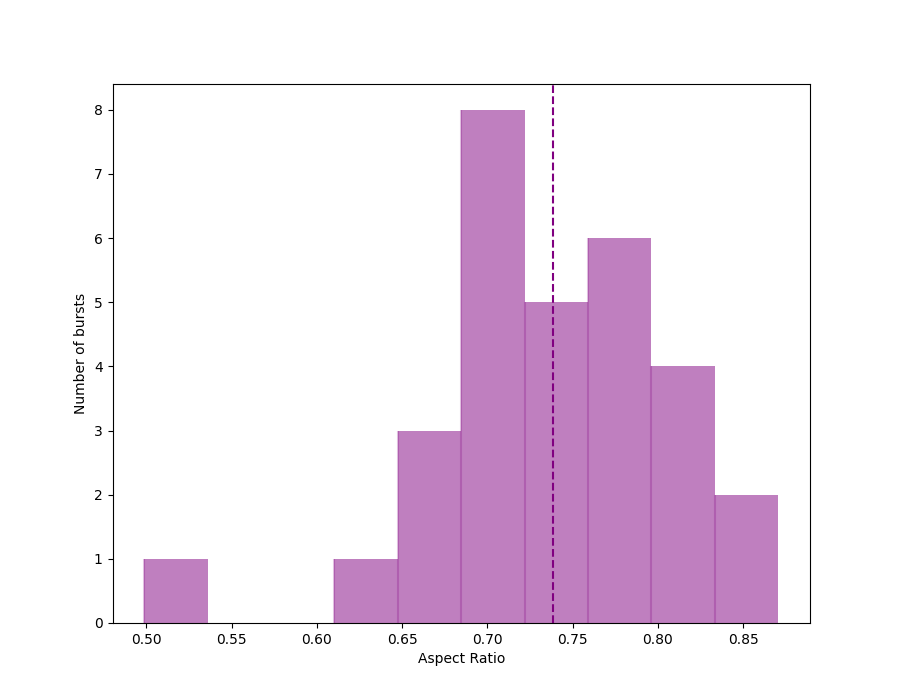
\includegraphics[width=\columnwidth]{burst_fwhm_ratio_histogram.png}
%\caption[Histogram of type III burst aspect ratios.]{Histogram of type III burst aspect ratios. The vertical purple dashed line indicates the mean value for the aspect ratio FWHM\textsubscript{x}/FWHM\textsubscript{y}.}
%\label{fig:fwhm_ratio_hist}
%\end{figure}
Figure \ref{fig:burst_hist}a shows a histogram of FWHM\textsubscript{x} and FWHM\textsubscript{y} in the range of 6 to 20~arcmin. The mean size of the bursts is indicated by a vertical grey dashed line and is $11.96$~arcmin for FWHM\textsubscript{x} and $16.27$~arcmin for FWHM\textsubscript{y}. The histogram of burst aspect ratios is shown in \ref{fig:burst_hist}b with the mean aspect ratio of the bursts $\sim 0.74$ plotted as a vertical dashed line. 
The relative angle of each burst i.e. the angle between the minor axis of the burst and a line from its centre to (0,0) in helioprojective-cartesian coordinates, is plotted as a histogram in Figure \ref{fig:burst_hist}c. These peak are around $\sim -10^\circ$ and have a mean indicated by a dashed green line at $-18.33^\circ$.

%\begin{figure}[ht]
%\centering
%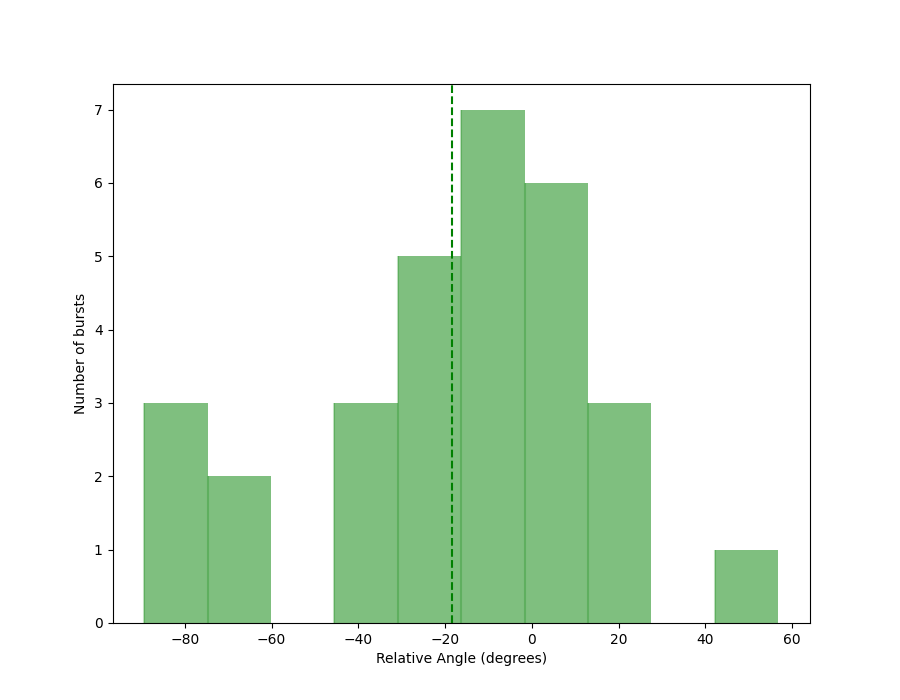
\includegraphics[width=\columnwidth]{burst_relative_angle_histogram.png}
%\caption[Histogram of type III burst relative angles.]{Histogram of type III burst relative angles. The vertical green dashed line indicates the mean value for the angle between the minor axis of the burst and a line joining its centre to (0,0).}
%\label{fig:rel_ang_hist}
%\end{figure}

\section{Discussion}
\label{sec:obsvtheory_discussion}
The observed source sizes of type III bursts are largely consistent with previous observations at similar frequencies in both interferometric and tied-array observations \citep{Kontar2017, Zhang2020}. In particular, the mean of the size in the major and minor axes is in agreement a previous measurement using the visibility fitting method \citep{Murphy2021}. As well as this, all 29 of the fitted bursts have an aspect ratio (defined above) of less than 1, which is suggestive of preferential scattering in a particular direction \citep{Anantharamaiah1994, Bastian1994}. The peaked distribution of relative angles in Figure \ref{fig:burst_hist}c is further evidence for alignment along a preferred direction. If this direction were radial, one would expect a peak around $0^\circ$ however here a mean value of $-18.33^\circ$ is observed. An examination of the magnetic field structure of the active region shows that some bursts are oriented such that their major axis is quasi-perpendicular to an open magnetic field line. These field lines are not necessarily radial with respect to the disk centre. Figure \ref{fig:pfss_overlay}a shows a good example of the previous statement. The burst, shown in blue contours, intersects with open magnetic field line, shown in yellow at a quasi-perpendicular angle. This is in agreement to observations of bursts in the solar wind \citep{Anantharamaiah1994, SasikumarRaja2016}. The assumption that the radio bursts are generated in open field lines above AR 12738 is only true for some of the bursts observed. There are a number of bursts that do not appear to be associated with the active region e.g. the burst in Figure \ref{fig:pfss_overlay}b. It is possible that such bursts originated behind the limb. %The large cluster of bursts in the north east corner of Figure \ref{fig:burst_overlay} shows bursts from when the active region is just behind the limb to when it rotates around.

\begin{figure}[ht]
\centering
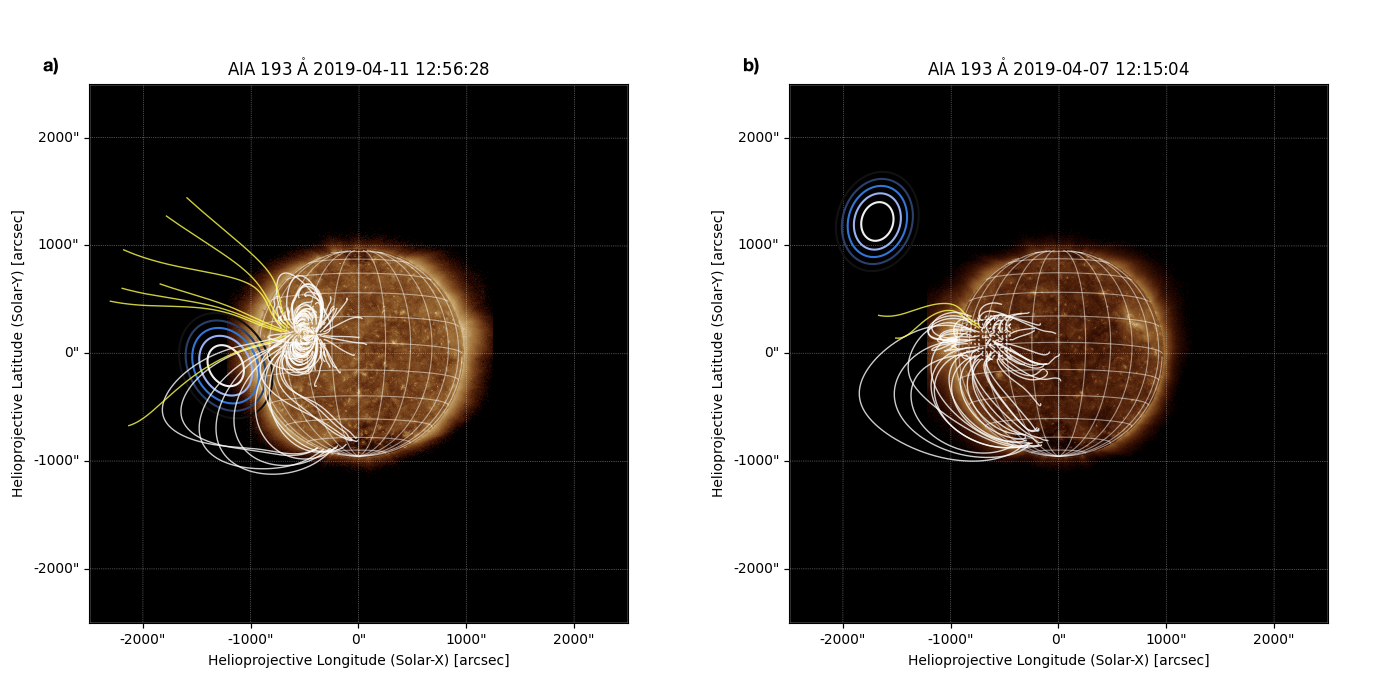
\includegraphics[width=\columnwidth]{pfss_burst_overlay.png}
\caption[Overlay of burst location with PFSS from active region 12738.]{Overlay of burst location with PFSS from active region 12738. The background image is an AIA 193 \AA \ image of the Sun at the time indicated in the title. Blue contours are the intensity of the radio burst from 50\% of the max value to 100\% in steps of 10\%. Open field lines are shown in yellow, white lines are closed field lines. Panel a shows the type III burst is oriented quasi-perpendicular to an open field line from AR 12738. Panel b shows a type III burst that is not associated with any open field lines from the PFSS and may have originated behind the limb.}
\label{fig:pfss_overlay}
\end{figure}

There is one major deviation between the model of scattering through anisotropic density fluctuations in a spherically symmetric corona and these results. \cite{Kontar2019} predict that, for a point source, the aspect ratio of a radio burst should decrease with increasing heliographic longitude, i.e. distance away from the disk centre along the solar equator. However, as shown in Figure \ref{fig:fwhm_comp}, no such trend is evident.  
There are a number of reasons why this may not be the case. Firstly, it is possible that calibration of the data did not fully converge or that the observation itself was corrupted. I believe this to be unlikely firstly because the Gaussian fit to each of the 29 bursts was manually inspected and any such flaw would be apparent. Secondly, the position and orientation of the bursts with respect to the magnetic field lines of AR 12738 agrees with the theory that type III bursts are generated along open magnetic field lines \citep{Wild1950a, Wild1950d} and are oriented with their major axis perpendicular to the field line \citep{Anantharamaiah1994}. 
Assuming the observation and data analysis are free from error, the simplest answer to why this is the case is mentioned in the discussion of \cite{Kontar2019}. They argue that the total observed size can be considered as the intrinsic size of a burst and the size due to scattering of a point source added in quadrature FWHM\textsubscript{total} = (FWHM\textsuperscript{2}\textsubscript{intrinsic} + FWHM\textsuperscript{2}\textsubscript{scattering})$^{1/2}$. Therefore, no trend in source sizes could suggest that type III bursts have an intrinsic size that is greater than the size due to scattering. 

\begin{figure}[ht]
\centering
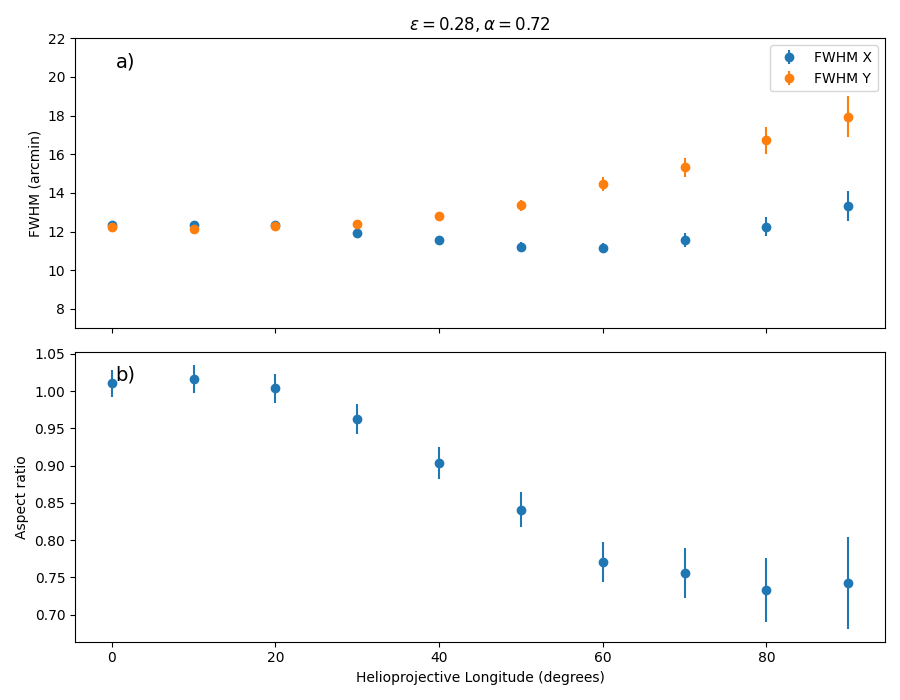
\includegraphics[width=\columnwidth]{fwhm_model_pj.png}
\caption[The modelled size and aspect ratio of a radio burst at 30.6~MHz.]{The modelled size and aspect ratio of a radio burst at 30.6~MHz. Panels a and b correspond to panels a and c in Figure \ref{fig:fwhm_comp} respectively, although here the x axis is heliographic longitude. The model was run with $\varepsilon = 0.28$ and $\alpha = 0.72$.}
\label{fig:model_comp}
\end{figure}

\begin{figure}[ht]
\centering
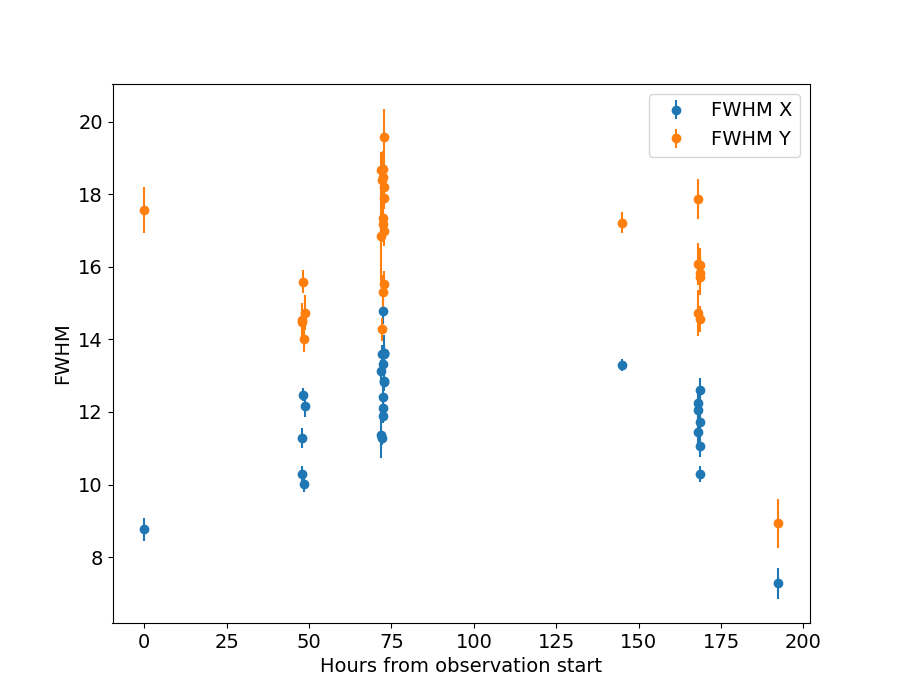
\includegraphics[width=\columnwidth]{fwhm_time_comp.png}
\caption[Plot of FWHM size of radio bursts with respect to time.]{Plot of FWHM size of radio bursts with respect to time. There is a spread of sizes in both FWHM\textsubscript{x} (blue) and FWHM\textsubscript{y} (orange) of the order of $\sim 5$~arcmin over the course of an hour which could be interpreted as temporal variance of $\varepsilon$ or $\alpha$ on timescales of minutes.}
\label{fig:fwhm_time_comp}
\end{figure}

An alternative explanation could be that the level of r.m.s fluctuations and anisotropy are different to what \cite{Kontar2019} suggest. The parameter space for the scattering model was explored by \cite{Zhang2021} who found that in order to match the observed decay time and size of a radio burst at 35~MHz, a value for r.m.s fluctuations of $\varepsilon = 0.28$ and an anisotropy factor of $\alpha = 0.72$ were necessary. The expected size and aspect ratio of a burst at 30.6~MHz were calculated using the Python version of the \cite{Kontar2019} scattering model from \cite{Zhang2021}. Figure \ref{fig:model_comp} shows the result of modelling a radio burst at different heliographic longitudes with the parameters suggested by \cite{Zhang2021}. It is immediately obvious that the modelling result does not match what is observed in the left column of Figure \ref{fig:fwhm_comp}. It also shows the opposite of Figure 8 in \cite{Kontar2019} whereby FWHM\textsubscript{x} remains roughly constant while FWHM\textsubscript{y} is seen to increase with increasing heliographic longitude. The expected trend towards smaller aspect ratios with increased heliographic longitude remains.
% (left column) and \cite{Kontar2019} (right column). It is immediately obvious that neither of sets of parameters matches what is observed in the left column of Figure \ref{fig:fwhm_comp}. 


%This explanation is less likely because the effect of anisotropic density inhomogeneities is most evident near the solar limb where the majority of the bursts were observed. Thus this is the most likely location to see a change in aspect ratio with respect to heliocentric angle but this is still not the case.

%The histogram of burst sizes in Figure \ref{fig:burst_hist}a shows that the minor size of the bursts are peaked around the mean whereas the major size is possibly double peaked. It stands to reason that the source size in the minor direction undergoes less scattering, therefore retaining its intrinsic size, than in the major direction where the size distribution is almost random.

%Perhaps a more damning indictment for all scattering models comes when one relaxes the assumption of a spherically symmetric solar corona that is constant in time.  If, as is widely accepted, radio burst generation is concentrated in open magnetic field lines above the active region seen in Figure \ref{fig:ar_evolve} then the spectrum of density inhomogeneities is sure to change as the active region evolves. The time scale for this change is clearly less than the order of a few days, otherwise the trend in aspect ratio should be observed in Figure \ref{fig:fwhm_comp}. A lower limit on this time scale is more elusive. Bursts observed over the course of one hour on a given day all share a similar size, orientation and aspect ratio which gives a lower limit of at least one hour. Thus it is reasonable to assume that the power spectrum of density inhomogeneities is constant on the order of a few hours but not for time scales over a number of days. The exact change to the power spectrum during this time remains unknown but is undoubtedly linked to magnetic flux emergence in the active region and it is likely that the assumption of constant $\varepsilon$ is also incorrect and that either the level r.m.s fluctuations change or the actual electron density of the emitting region changes.

 %This agrees with my suggestion that $\alpha$ is larger than first suspected by \cite{Kontar2019} however, the frequency dependence of $\alpha$ has not been examined here.
The modelling in this analysis was performed under the assumption that $\varepsilon$ and $\alpha$ do not change with time or position in the solar corona. Neither of these assumptions are necessarily true. Considering that burst orientation is strongly related to the local magnetic field line direction, it is possible that there is spatial variability in these measures of coronal turbulence. To investigate any possible temporal variance of $\varepsilon$ and $\alpha$, the FHWM size in the helioprojective-cartesian x and y direction are plotted with respect to time in Figure \ref{fig:fwhm_time_comp}. Over the course of an hour the FWHM size of the burst varies by $\sim 5$~arcmin while the biggest difference in source size over the entire observation is $\sim 8$~arcmin and $\sim 11$~arcmin for FWHM\textsubscript{x} and FWHM\textsubscript{y} respectively. If the observed source size were \textit{only} due to scattering then any change may be indicative of temporal variability in either $\varepsilon$, $\alpha$ or both.



%The absolute x positions in the range 0 - 1000 arcsec and absolute y positions in the range 0 - 200 arcsec are possibly under sampled compared to the dense cluster of bursts observed around -1500 arcsec, 750 arcsec. The reason for this discrepancy, while not justifying it, is because of poor calibration of the interferometric visibilities as the radio noise storm became more intense. This coincided with the active region rotating to the centre of the solar disk and thus poor sampling in this region. That said, repeating the above analysis with bursts fitted even though there is poor calibration returns much the same result although with greater scatter and error, as one might expect. Therefore, even though the bursts shown in this chapter may not fully sample the space, they are properly representative of radio bursts in general. %I also reiterate the point made above that the effect of scattering on source size is more evident near the limb which is well sampled. 

\section{Conclusion}
Observations of the position and size of 29 type III radio bursts do not fully agree with results from models of radio wave scattering in the solar corona. After thorough inspection of interferometric calibration and fits to interferometric visibilites, I attribute this discrepancy to an intrinsic source size of type III bursts. Work needs to be undertaken to improve the calibration procedure for solar radio bursts so that the initial sample of $\sim 300$ bursts can be analysed. 
The scattering model used in this analysis assumes a spherically symmetric, unmagnetised, corona \citep{Kontar2019, Zhang2021}. Most of the bursts in this analysis are seen to be located above the active region AR 12738 which has a much greater electron density and magnetic field strength than the quiet corona. Thus, changes to the electron density model and including the effects of magnetic fields may be necessary to explain the difference between observations and the results from scattering models.

Before one can use observations of radio bursts to determine the physical parameters of coronal plasma and the radio wave scattering process, the discrepancies between the results presented here and previous modelling work must be addressed. Improvements to interferometric calibration techniques and including the effects of magnetic fields and active regions in scattering models are the two most prominent issues in this regard. %begin to distinguish the variability of the suggested intrinsic source size of a type III burst determined in this work from the variability due to scattering

In this chapter I outlined the development of scattering models for radio waves in the solar corona from seminal works to modern day advancements. I also stated the importance of comparisons between these models and contemporary observations. I then detailed the observation of hundreds of type III radio bursts during a radio noise storm over the period 04 April 2019 to 14 April 2019. Using LOFAR interferometric visibilities at $\sim 30$~MHz and a method similar to \cite{Murphy2021}, I fit 29 of the calibrated bursts to determine their size and shape. I found that type III radio bursts have a mean size in the minor and major axis of $11.96$~arcmin for and $16.27$~arcmin respectively and a mean aspect ratio of 0.74. No trend in aspect ratio with respect to burst location was evident in the observations and as such, I attributed this to the intrinsic size of type III radio bursts being greater than the size due to scattering. The relative angle between the minor axis of each burst and a radial line from the centre of the Sun to its centre has a mean value of $-18.33^\circ$ and indicates preferential orientation. The magnetic field was modelled using a PFSS model and the source orientation was found to be perpendicular to open magnetic field lines for some of the bursts. Using the mean values achieved as a typical intrinsic size agrees well with previous observations with LOFAR in both interferometric and tied-array images at similar frequencies. This work is \textit{in prep} for submission to \textit{Astronomy and Astrophysics}.
